\chapter{Background}
Some context and knowledge is required for understanding the task at hand. It is assumed that the reader has some knowledge on the topic of spatial data, but a brief intro will be given in this chapter. For a more detailed explanation of spatial data and its underlying data structures, materials such as \textit{The Design and Analysis of Spatial Data Structures} is recommended \cite{spatial_data_structures}.
\section{Spatial Data}
Spatial data is simply data that contains spatial properties in some shape or form. These can include, but are not limited to, points, lines, rectangles, regions, surfaces and volumes \cite{spatial_data_structures}. There can be additional data present, but that is not a requirement. One of the most common data types to pair with spatial data is temporal data. This is known as spatio-temporal data, and is used extensively throughout the world. One interesting effect of storing spatial and temporal data together is that you can create trajectories, essentially drawing a line from the starting point, through all the intermittent points and to the end point. But how does one know when to generate a point? The two most common methods are to either save the location at a set time interval, or to save the location after a set distance interval. Another way, commonly used by apps such as Google Maps, is to save the location when the user stops and spends time close to a point of interest. These points of interests can be anything from statues to cafés. From this you can see how long each stop is, the average movement speed, where the user spends most of its time and generate patterns in user movements. \\

To limit the scope of this project, we will not focus on the temporal part of the data. We will instead only look at the spatial properties, such as the coordinates, but we can use the temporal properties to induce an ordering the the points, creating a linked directional property to each trajectory. We will also not focus on spatial data with more than two dimensions or look into different types of databases.

\section{Dataset}
There are quite a few different datasets publicly available that would be suitable for this project. To determine which datasets were relevant we would need to look at different aspects and see if they have everything we need. These aspects include:
\begin{itemize}
	\item \textbf{Spatial properties.} \\ For the dataset to be relevant at all it needs spatial properties. Either GPS coordinates or another X,Y system.
	\item \textbf{Be based on real-world data.} \\ Real-world data makes the data points more genuine and realistic. Generating a new dataset could also be used, but that might not take into account different aspects one would get with real-world data.
	\item \textbf{Some kind of ordering.} \\ This can either be through having links between data points, implicit ordering from the rows of the file, or inductive ordering through timestamps.
	\item \textbf{Sufficient data.} \\ A dataset of a few kilobytes is not going to be enough data to make sure that the evaluation works. A few gigabytes would be optimal, but a a little less than one gigabyte should be sufficient as well.
	
\end{itemize}

\subsection{Dataset Providers}
There are several companies that use spatial data. Companies such as Strava have built empires using, manipulating and mining spatial data. Initially, Strava was looked at in case they had any anonymized datasets available. Being that largest fitness tracking app in the world, they would surely have some data available, right? Unfortunately, not without some caveats. To access their data, one would have to use their API. This is an open API, but it would require explicit consent from a lot of users to get a feasible amount of data. In addition, Strava does impose quite a lot of restrictions on how the dataset is used and distributed. These restrictions posed too much of a hassle to make it a viable option. \\

Kaggle is a community for data science and machine learning. They regularly host competitions where users are provided a dataset and have to create the best algorithm to solve a problem. These datasets are not created by Kaggle themselves, but rather provided by companies, users or researchers. Throughout Kaggle's history there have been several competitions, and as a result there are a lot of datasets available for download. As these are used for different competitions they consist of all types of data and sizes. Some datasets are only a few kilobytes in size whilst others are several gigabytes. Fortunately, they have a search functionality that allows you to filter datasets based on several different factors, including size, date, data type, and others. Table \ref{tab:datasets} shows some of the datasets that were considered. In the end, the Taxi Trajectory Prediction dataset was chosen. It fulfilled all the requirements, whilst also being really descriptive and easy to understand. This dataset was also recommended by Svein Erik Bratsberg during the initial meeting for this project.
\begin{table}
	\centering
	\label{tab:datasets}
	\caption{Datasets that were considered from Kaggle.}
	\begin{tabularx}{\textwidth}{|X|X|X|X|X|} \hline
		\multicolumn{1}{|X|}{\textbf{Name}} & \multicolumn{1}{X|}{\textbf{Spatial Properties}} & \multicolumn{1}{X|}{\textbf{Real-World Data}} & \multicolumn{1}{X|}{\textbf{Ordering}} & \multicolumn{1}{X|}{\textbf{Sufficient Data}} \\ \hline
		Microsoft Geolife GPS Trajectory Dataset & Yes & Yes & Timestamped & Yes - 1.67 GB \\ \hline
		T-Drive Trajectory Dataset & Yes & Yes & Timestamped & No - 803 MB \\ \hline
		GPS data from Rio de Janeiro buses & Yes & Yes & Timestamped & Yes - 6 GB \\ \hline
		Wrocław public transport & Yes & Yes & Timestamped & Yes - 3.56 GB \\ \hline
		ECML /PKDD 15: Taxi Trajectory Prediction & Yes & Yes & Polyline & Yes - 533.7 MB (compressed) \\ \hline
		
	\end{tabularx}
	
\end{table}

\section{Existing Data Structures for Spatial Data}\label{sec:data_structures}
Spatial data is not a new concept. As early as the 1960's research began on studying geographic information systems (GIS) \cite{history_gis}. However, as the amount of spatial data has increased significantly over the past few years, spatial data has become more relevant than ever. The most common way to store and work with spatial data is through spatial databases. These are databases that are specifically designed to store and perform queries on spatial data. Although they are commonly referred to as spatial databases, none of the commercially available and well-known spatial databases are exclusively spatial-oriented. They are all plugins and extensions built on top of existing databases, or simply a small part of a DBMS. Perhaps the most known spatial database is PostgreSQL with the PostGIS plugin. \\

For a spatial database to store and query spatial data there needs to be some properties present. The most important one being the spatial indexing method, as that is essential for querying spatial data effectively. Normal databases use indexes such as B$^{+}$-trees, but these are no good for querying spatial data. Most spatial database systems allow for using different indexing methods based on what the user needs, but the most common indexing method is R-trees or any of its variants. The different indexing methods all take different approaches and allows for different amount of dimensions to their data. Some prioritize dynamic data, data that will change during the usage, and some prioritize static data. When prioritizing dynamic data, an index method must easily be recreated or updated to accommodate the changes. If it takes a long time to adapt to the changes, the queries to the data will be slow and will result in a bad experience for the user. If one knows that there is not going to be any changes to the data, one can go for an indexing method that might use more time to generate the index, but has a faster time for querying the data after the index is up and running. \\

There are two main categories for the data structures used by spatial indexing methods: space-driven and data-driven structures. Space-driven structures divide the entire space into zones based on the data present. Some examples of this include quadtrees and kd-trees. Data-driven structures on the other hand do not divide the entire space, but rather uses the data to only create zones that are encompassing the data, using only the minimum amount of space required. This category contains R-trees and all its variants. \\

Different indexing methods can also be faster for some types of queries and slower for others. The \textit{Open Geospatial Consortium} has defined some predicates which indicate how geometries interact with each other \cite{spatial_predicates}. These, and others, are often built into the spatial databases such that users do not have to write custom functionalities for them.

\subsection{Quadtrees}
Quadtrees are a space-driven data structure used for indexing two-dimensional spatial data. They work by dividing the space into four squares, and then dividing those again until you only encompass a set amount of points in each square. There are several variations of quadtrees as they are used for different use cases such as image compression, storing polygons and several others. The different variations include point-, region, point-region-, PMR- and XBR quadtrees \cite{quadtrees}. In figure \ref{fig:quadtree} you can see a point-region (PR) quadtree represented as both a grid based on the position of the points as well as a tree. For connected directional spatial data the most relevant quadtrees to look at would be the point-region-, PMR- and XBR quadtrees.

\begin{figure}
	\centering
	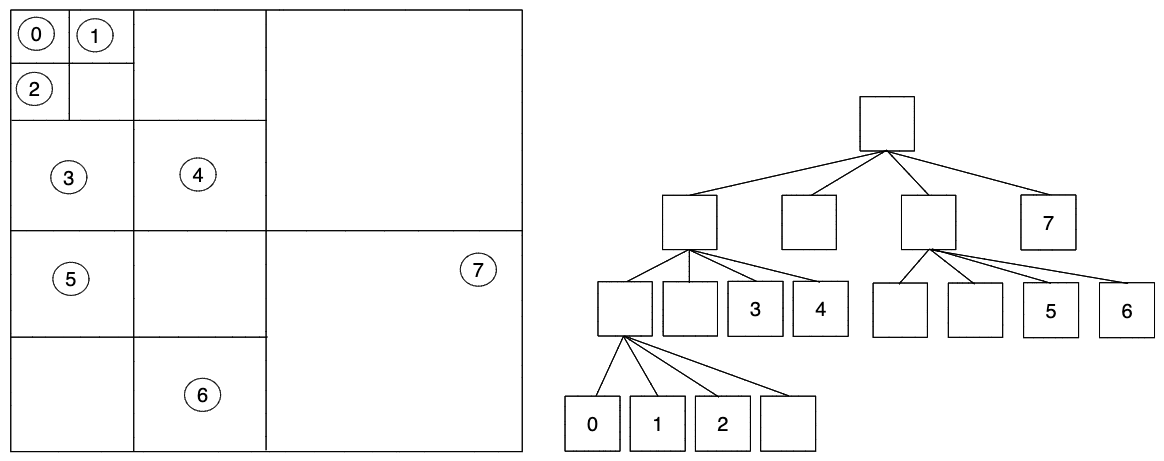
\includegraphics[width=\textwidth]{figures/quadtree.excalidraw.png}
	\caption{A PR quadtree with seven points and a maximum of one point per cell represented as both a grid and a tree.}
	\label{fig:quadtree}
\end{figure}

\subsection{R-trees}
R-tree is a data-driven structure invented in 1984 by Antonin Guttman that is used for indexing multi-dimensional data \cite{r_trees}. The concept is closely related to B$^{+}$-trees, but the data is grouped by its spatial properties. It works by grouping items by using \textit{minimum bounding rectangles} (MBR). MBRs are the smallest possible rectangles one can create for a set of objects whilst enveloping their coordinates. By grouping data with MBRs, one can easily query the data on their spatial properties by looking at the MBR and seeing if the rectangle satisfies the constraints of the query. With R-trees there are rectangles \textit{all the way down}, meaning that several MBRs are grouped by a larger MBR with the data contained in the leaf nodes. \\

Throughout time there have been many proposed variations of R-trees, with a few of them being used extensively. R*-trees were first proposed in 1990 and improves on the original concept. In essence, the R*-tree uses more computational power to create trees with less overlap and smaller MBRs. This allows for better query performance than the original R-tree. The R$^+$-tree does not allow overlapping MBRs on the same level, causing greater performance for point queries, but worse performance for window queries due to storing duplicates rather than overlapping MBRs. In addition to these variants there are several others that do their own optimizations and concessions in order to improve the performance in some regard. A more detailed and comprehensive list of R-tree variations can be found in \cite{r_tree_variations}.


\subsection{Comparing R-trees and Quadtrees}
A study done by Oracle in 2002 found that R-trees are faster than quadtrees for querying of almost all types. R-trees were faster for \textit{anyinteract, inside, contains, touch, coveredby, covers, equals, overlapbydisjoint}, and \textit{overlapbyintersect}. However, quadtrees were better for \textit{touch, overlapbydisjoint,} and \textit{overlapbyintersect} \underline{only} when using larger query windows. They also found update times to be better for R-trees and storage requirements similar for both structure, but only when using points. For everything else R-trees outperform quadtrees. Essentially, they recommend using R-trees unless you are creating 
\begin{quote}
	\textquote{[...] update-intensive applications using simple poly-
gon geometries, high concurrency update databases,
or when specialized masks such as touch are frequently
used in queries.} \cite{oracle_comparison_quad_vs_r}
\end{quote}

They also found that using quadtrees required a lot of fine-tuning to reach optimal performance. This is not required for R-trees and provides R-trees with another advantage. \\

Out of all this, we can gather that the different data structures have their own advantages and use-cases. For this project it can be beneficial to keep both in mind look at how the different aspects can be used for making an optimal data structure for querying linked directional spatial data.

\subsection{Space-filling Curves}
Space-filling curves (SFCs) are mathematical functions used to map multi-dimensional data points to a single dimension whilst preserving the spatial relationships of the data points. They only access each location once, and never crosses itself \cite{hilbert_r_tree_original}. SFCs have several applications including image compression, computer graphics and spatial indexing. \\

There are several different variations of SFCs, with the most well-known being the Hilbert curve which was described in 1891 by David Hilbert \cite{hilbert_curve}. It is preferred over other curves, such as the Morton curve, as it better preserves the spatial relationships between points \cite{spatial_data_structures}. \\

Space-filling curves can be utilized in spatial indexing either alone or accompanied by either a space-driven or data-driven structures such as the ones introduced previously. The Hilbert R-tree is a famous variation of the R-tree that utilizes the Hilbert space-filling curve to better preserve the locality of the data points than the original R-tree in case of splits. Space-filling curves can also be used in conjunction with quadtrees as can be seen in figure \ref{fig:space_filling_curve}.

\begin{figure}
	\centering
	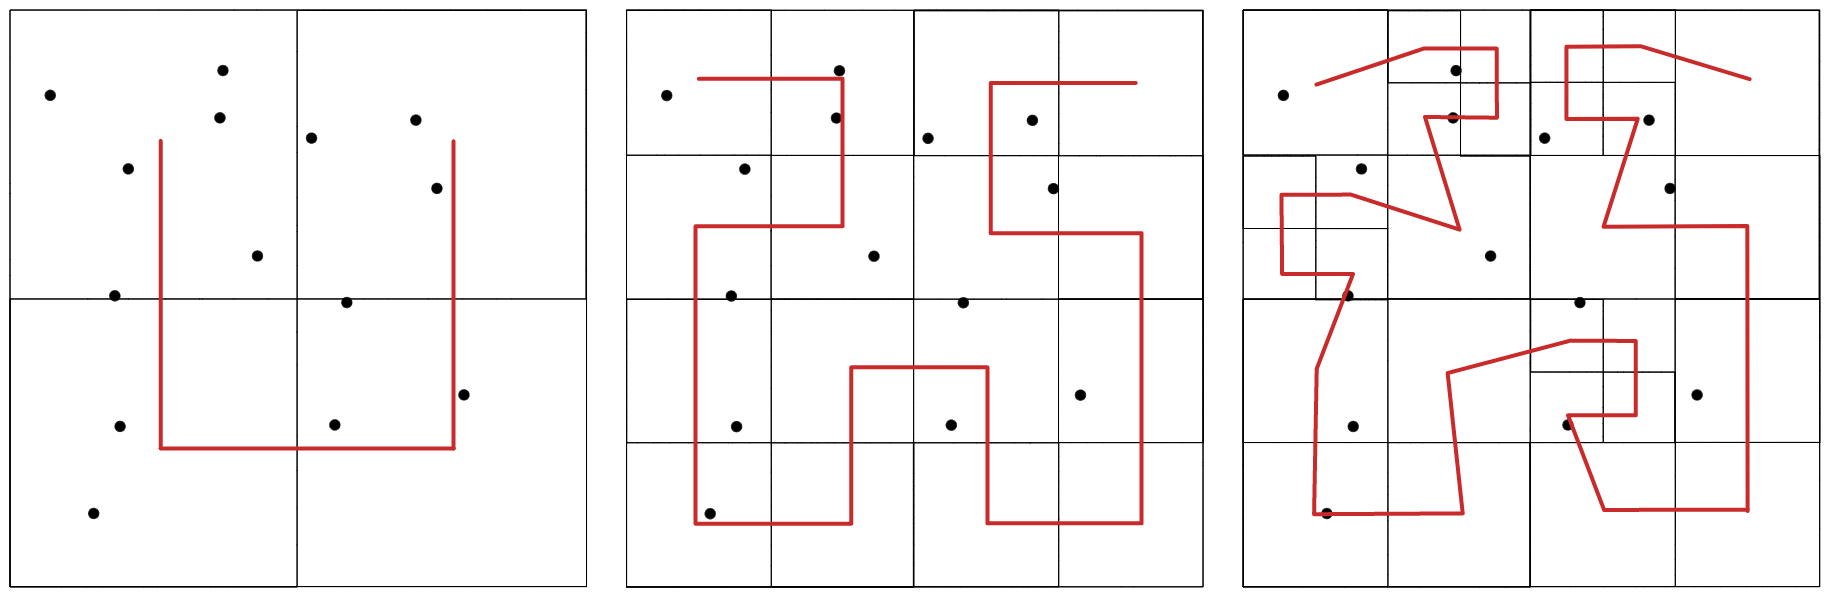
\includegraphics[width=\textwidth]{figures/space_filling_curve.excalidraw.png}
	\caption{Hilbert space-filling curve used with a quadtree. Note how the depth of the quadtree affects the order of the curve.}
	\label{fig:space_filling_curve}
\end{figure}

\section{Linked Lists}
Linked lists are a common data structure in computer science and are used in several. It consists of nodes linked together with pointers pointing from one node to the next. They do not use indexes as the nodes can be stored anywhere in memory, with only the pointers telling where the data is. Because of this, one can not access any given node directly, but you rather have to traverse the list from start to finish to read items. Why are linked lists relevant? Linked directional data is essentially just linked lists containing spatial properties. There are nodes which are logically connected to other nodes through some kind of ordering.Utilizing linked lists for spatial data is not an original thought and has been used in MX-CIF quadtrees previously all the way back in 1982, but luckily in a different way from what we are proposing here \cite{spatial_data_structures}.

\subsection{Expanding Linked Lists to Accommodate Spatial Data}
Linked lists work fine, but up against data structures as R-trees they are quite simple. Using standard linked lists will not use the spatial component of the data, which is needed to make efficient queries. To differentiate this data structure from linked lists, we will refer to it as \textit{linked MBR lists}. This name is temporary and should be revisited at a later date to find something more fitting that takes into account all aspects of the data structure.

\subsubsection{Adding MBRs to Nodes}
To expand the linked list we can add an MBR to each node, which also encompasses all of its children. For this to work, one would have to have a doubly linked list as the MBR will have to be created from the bottom up. A visualization of the data structure can be seen in figure \ref{fig:linked_mbr_list_in_python}. \\

Adding MBRs to each node will allow for easily determining if a query window intersects the MBR of the head, which tells us from the first node if the query can or can not be satisifed from this list. Also, by having the MBR of all later nodes in each node, we can terminate the traversal when the MBR no longer intersects a query window or encompasses a query point. This works well when the query window is close to the head of the list, but if only the last node is within the query window this would still result in traversal of the whole list.

\begin{figure}
	\centering
	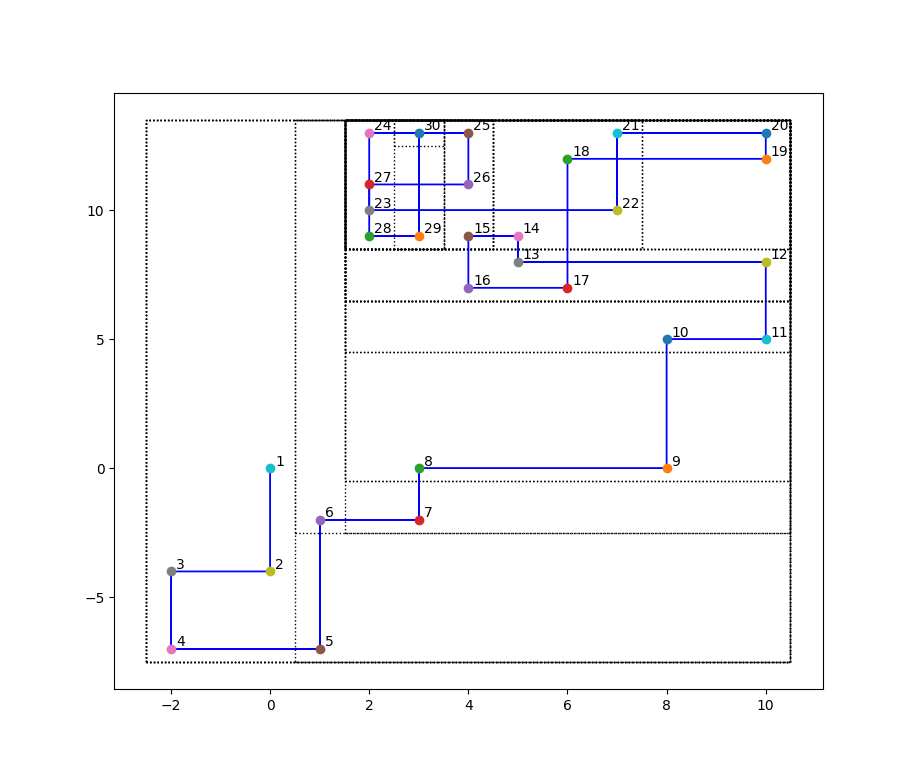
\includegraphics[width=\textwidth]{figures/linked_MBRs_python_example.png}
	\caption{Visualization of MBRs added to each node. The MBRs are shown in dotted rectangles.}
	\label{fig:linked_mbr_list_in_python}
\end{figure}

\subsubsection{Skipping Nodes Based on Distance}
By adding MBRs to each node one can more efficiently query on the spatial properties of the data. However, this does not utilize the linked aspect of the linked list. When querying one would have to traverse each node, checking if the node itself is within the query window, and then checking if the MBR intersects the query window. These are not heavy computational checks, but they do add up over a large amount of nodes. One way to skip these checks, only traversing until a specific node, could be done by calculating the maximum distance between any two consecutive nodes in the list $M$. By knowing the maximum distance that occurs between two consecutive nodes within the list, one could look at the head node, check the distance from it to the closest point of the query window $D$, and if $D > M$ one could traverse $S = floor(D/M)$ nodes without checking neither the node's location or their MBR. After having traversed $S$ nodes, one could check the location of this node and do the calculation again. If $D > M$ still holds true, one could traverse $S$ nodes again without checking. The cycle repeats until $D > M$ is false.

\begin{figure}
	\centering
	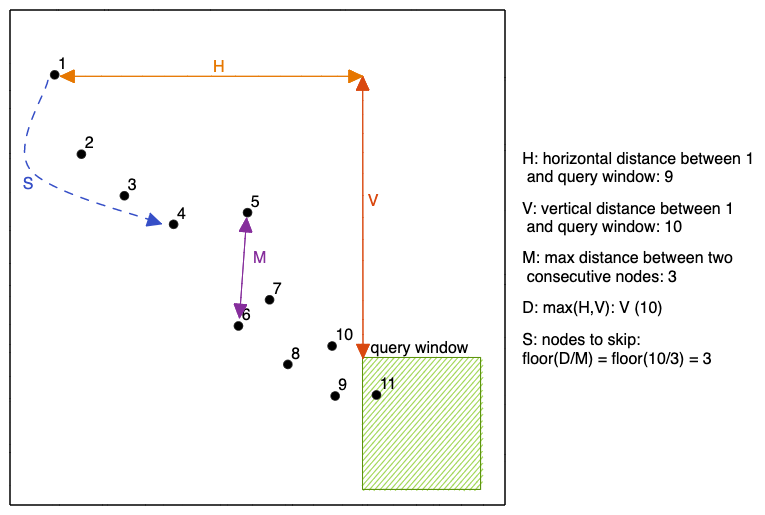
\includegraphics[width=\textwidth]{figures/node_skipping.excalidraw.png}
	\caption{Visualization of node skipping based on distance. Note that one would still have to traverse from node 1 $\rightarrow$ node 2 $\rightarrow$ node 3 $\rightarrow$ node 4, but one would not have to check their spatial properties or MBRs.}
	\label{fig:node_skipping}
\end{figure}

\subsubsection{Skipping Nodes Based on MBR Change}
One unfortunate aspect of the linked MBR list can be seen in \ref{fig:linked_mbr_list_in_python}. Node 1 and node 4 have the same MBR. Node 1 is laterally dominated by node 4 and node 20 and longitudinally dominated by node 4 and node 30. This would store the same MBR on several nodes, causing superfluous lookups. One way to prevent these redundant checks would be to add pointers between nodes where there are no changes in MBRs upon creation. This would allow for traversing the nodes, checking them against the query window, but without having to check the MBR for each one. \\

For instance, in figure \ref{fig:linked_mbr_list_in_python} one could add a pointer from node 1 $\rightarrow$ node 4 as they both have the same MBR. The same could be done from node 12 $\rightarrow$ node 17 as the MBR does not change between those either. Adding these extra pointers would require expanding the data structure even further from a linked list, adding an optional pointer. For the example used here, it would not save much time or many steps, but for a large trajectory where the MBR does not change for a significant amount of nodes, this could save some time.

\subsubsection{Indexing}
Currently, if you were to query these lists you would have to check the MBR of each individual list as an initial filtration. This is obviously bad for performance, and an indexing method would be needed for mitigating this. Trees are effective as they effectively prune large amounts of data on the first split, with balanced binary trees pruning half the data initially. To prune data early we need to divide the search space into zones. We have already seen that existing methods use space-driven and data-driven structures for dividing the search space. Our current implementation is data-driven as the MBRs are generated out of the data itself. One idea would be to implement a space-driven structure on top of the linked MBR lists. This would create a hybrid structure where the initial splits would be done on the search space until there is only one MBR in each reactangle and further divisions would be done by the MBRs. \\

The big question when implementing the space-driven aspect of the structure is what algorithm is to be used. Although kd-trees are generally preferred for static data, the fact that splits the data in two, as it is a binary tree, makes it conflict with the MBRs as that would split the content of the MBR into separate buckets. Because of this, despite the fact that we are using static data, quadtrees are to be preferred here. A point quadtree would be impractical as it is a binary tree adaptation and would split the MBRs in the middle in the same manner as the kd-trees. A point-region quadtree would work.

\subsubsection{Splitting Trajectories}
Another optimizations that can be done is to split the MBRs of the trajectories. This will keep the pointers from one node to another, but the MBR will be reset at some point during the chain. To keep the MBR of the entire trajectory, an extra node will be prepended to the linked list, not containing any point, but rather just the MBR of the entire path and pointers to the first nodes in each split. What this allows for is splitting the trajectory on where the two resulting MBRs would be the smallest and removing the most amount of dead space where there are no points. How many times this should be allowed can be used as a tweakable parameter, allowing for tailoring it to each dataset. One could also have the amount of splits dependant on a set variable so that all splits would contain a set amount of nodes.  A visual comparison of a list without trajectory splitting and with a single split can be seen in figure \ref{fig:trajectory_splitting}.

\begin{figure}
	\centering
	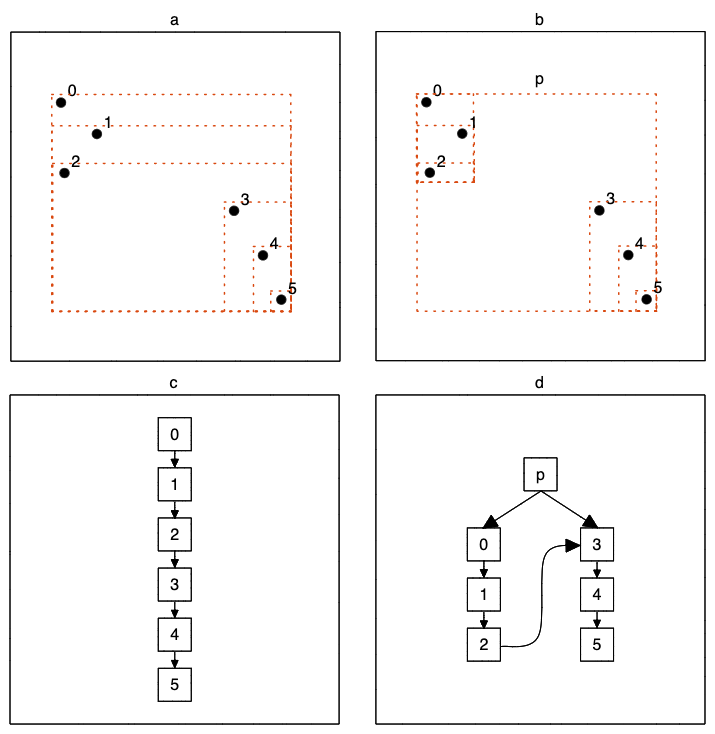
\includegraphics[width=\textwidth]{figures/Trajectory_splitting.excalidraw.png}
	\caption{Visualization of splitting trajectories once. $a$ and $b$ show how the MBRs will be affected and $c$ and $d$ show how the linked list will be affected. Node p is a node that is not a point, but rather the parent MBR of the entire list.}
	\label{fig:trajectory_splitting}
\end{figure}

\subsection{Querying Linked MBR Lists} 
How querying linked MBR lists would work is dependant on the top-level indexing method. For now we will assume that we are using a point-region quadtree and that the query is \textit{is contained by} with a query window $q$. Querying would work by first narrowing down the search space to the smallest possible quadrant(s) in the quadtree. From there, each top-level MBR (MBR of the first node or the parent MBR $p$) would be checked against the query window and if they are disjoint it would be discarded. If there are any top-level MBRs that are not disjoint their lists will have to be traversed. If the MBR is a parent MBR, it will check the MBR of its first child first, and if it is disjoint it will skip to the next child without traversing the children of the first child. For instance, in figure \ref{fig:trajectory_splitting} we assume that the MBR of $p$ intersects the query window, but the MBR of node 0 does not. Then, node 0 through 2 would not be traversed, but one would rather go directly from $p$ to node 3. This continues until one of the MBRs intersects the query window. Once an intersecting MBR is found the traversal of the list would begin. The distance from the first node to the query window would be calculated and if the distance is greater than 0 the corresponding amount of nodes would be traversed without checking the MBR. If any node in the traversal is enveloped by the query window it will be appended to the list of results. If the MBR of any node is disjoint with the query window the traversal would terminate and result list is either returned, or if there are more intersecting trajectories the next trajectory is traversed.

\begin{comment}
	
\begin{algorithm}
	\caption{Creating MBRs in a linked MBR list (TO BE CHANGED TO UTULIZE NODE SKIPPING)}
	\begin{algorithmic}
		\State $n \gets N.last$ \Comment Start with the last node in the list N
		\State $n.northWest \gets (n.x, n.y)$
		\State $n.southEast \gets (n.x, n.y)$
		\While {$n.parent \neq null$}
			\State $p \gets n.parent$
			\State $p.northWest \gets (Min(n.northWest.x, p.x), Min(n.northWest.y, p.y))$
			\State $p.southEast \gets (Max(n.southEast.x, p.x), Max(n.southEast.y, p.y))$
			\State $n \gets p$ \Comment Set the parent as the current node
		
		\EndWhile

		
	\end{algorithmic}
	\label{alg:creating_mbr}
	
\end{algorithm}

\begin{algorithm}
	\caption{Searching in a linked MBR list (TO BE CHANGED TO UTILIZE NODE SKIPPING)}
	\begin{algorithmic}
		\State \textbf{set of nodes} $result \gets \emptyset$
		\State \textbf{query window} $w$
		\State $n \gets N.first$
		\While{$n.mbr \cap w.mbr =$ true}
			\If{$n \in w.mbr$}
				\State $result.add(n)$
			\EndIf
			\State $n \gets n.child$
		\EndWhile
		\State \Return $result$	
	\end{algorithmic}
	\label{alg:searching}
	
\end{algorithm}

\end{comment}

\subsection{Limitations of linked MBR lists}
As this data structure is focused on querying static data, no compromises have been made to ensure that it is fast to update. Due to the amount of MBRs that are dependent on each other, inserting, deleting or moving nodes is going to be inherently computationally expensive. Obviously, being slow to generate is going to be a drawback in most real-life scenarios, but in a perfect world where the data does not change and in theory this should be fine. If the generation time is heinous it will not be usable, but time will tell. \\

One other limitation is that geometric tests against MBRs can be done in constant time \cite{spatial_access_methods}. This means that improvements such as node skipping might have an almost insignificant impact on performance. If this proves to provide next to no performance boost it can easily be stripped from the implementation. \\

Another limitation is that of how the indexing method will behave based on the dataset. Using a quadtree for structuring the data can cause issues as the data might have significant overlaps due to the nature of how the traffic flow of a city behaves. However, this should be mitigated by the trajectory splitting, but it can be something to be aware of during benchmarking.  \\

The possibly largest limitation of the linked MBR list is that the main bottleneck of databases is usually I/O.
This means that optimizing locality of the data is going to have the most impact. That is why R-trees store their data the way they do. Each node is one page, meaning that all the data within that node is contained to a single page on disk, making it really fast to access other data within the same spatial area as they are also close on disk. Now, if everything is done in-memory, this will not be relevant, but if it is to be implemented in a database this might affect performance. Knowing if this is a limitation without having put it into practice is not easy. \\

Overall, this data structure has quite a lot of components and small moving parts that can impact performance. In addition, data structures can behave very differently based on datasets (bound by the time complexity). The easiest way to see how well the method performs is to test it out.

\section{Evaluating Linked MBR Lists' Performance}\label{sec:evaluation}
Evaluation of the performance of linked MBR lists can be done in two ways: writing an extension to a spatial database that utilizes this data structure and see how it compares to existing indexing methods, or writing an implementation for both linked MBR lists and already proven data structures in some programming langauge and comparing the performance without using a database at all. \\

The queries that are of interest are the ones defined by \textit{Open Geospatial Consortium} as briefly mentioned in section \ref{sec:data_structures}:
\begin{itemize}
	\item \textbf{Disjoint}
	\item \textbf{Equals}
	\item \textbf{Touches}
	\item \textbf{Crosses}
	\item \textbf{Contains}
	\item \textbf{Within}
	\item \textbf{Covers}
	\item \textbf{Covered by}
	\item \textbf{Overlaps}
	
\end{itemize}

These are commonly known as \textit{DE-9IM} and the explanation of each predicate can be found in \cite{spatial_predicates}. Although it is supposed to be optimized for querying it can also be of value to see how it compares when it comes to generating the index and how much space the index takes up.

\subsection{Comparison Within a Database}
Comparing the performance of linked MBR lists in a spatial database would require writing an extension that allows for using alternative indexing methods. The spatial database with the most support for writing extensions is PostgreSQL. Extensions in Postgres is one of the main draws to the DBMS. Extensions can be used for creating new data types, modifying how a process is performed and, essentially adding functionality to the DBMS. These extensions can be written in different languages depending on what part of the DBMS one is altering. Adding new data types or operators can be done with SQL, whilst more advanced alterations must be done in low-level languages such as C or Rust with C being the standard. Even though Postgres has quite and extensive documentation on extensions, there is no official documentation on how to create an extension that adds an indexing method as it is only referenced in the \textit{CREATE INDEX} documentation:
\begin{quote}
	\blockquote{\textit{PostgreSQL provides the index methods B-tree, hash, GiST, SP-GiST, GIN, and BRIN. Users can also define their own index methods, but that is fairly complicated.}} \cite{postgres_create_index}
\end{quote}

Other sources on the topic are scarce, and it seems the general consensus on the topic is that it is not something that can be easily accomplished. One way to peek into what the process of creating a new indexing method looks like can be found by reading through the source code of available extensions that do create its own indexing methods. The source code of PostGIS is mirrored on GitHub\footnote{\url{https://github.com/postgis/postgis}}, and is publicly available. Taking a look at the file \textit{postgis/gserialized\_gist\_nd.c} we can look through what seems to be the implementation of R-trees. This implementation is only one of many files in the repository required for making spatial indexing work. Now, it is hard to distinguish what is the minimal amount of work is required for getting a custom indexing method up and running without having to understand all the code in the repository and having a deep understanding of the Postgres source code.

\subsection{Comparison Outside a Database}
The alternative to writing a custom indexing method in Postgres is to implement linked MBR lists in a programming language and comparing its performance to an already proven indexing method outside of a database. There are several programming languages that have indexing data structure implementations through libraries such as the R-tree package in Python \cite{python_r_tree}. However, implementing linked MBR lists in Python and comparing it to the performance of such a package would not be a fair comparison as this package is a wrapper for a C implementation, and C is a much faster language than Python \cite{cython}. One solution would be to write both data structures from scratch, making sure that the playing field is even when it comes to underlying technology. Deciding on which language to use depends on what the goal is. If both indexing methods are implemented in the same way without using any performance gains through means such as compiling to lower-level languages, this will show how the data structures compare relative to each other. This can be done in any programming language, either high-level or low-level with the same result. If the data structure is to be used in a database at a later stage it can be beneficial to write it in a low-level language such as C++, C or Rust, but if that is not a priority a higher level language can be used for development speed. \\

Comparison outside of a database would also require writing the queries for the benchmarks. 

\subsection{Result}
Both these comparison methods come with their own advantages and drawbacks. One one hand, an in-database implementation would be beneficial to see how each of them perform in a real-world scenario. This would allow for seeing if the algorithm has any benefit at all compared to how the currently implemented spatial indexing methods. It would also allow for seeing how I/O affects the performance. The drawback of this method is that it would require a significant amount of time and work to only get the indexing method implemented into a spatial database to start with before starting to benchmark the performance. If the indexing method is useless, this would be a waste of time. \\

Writing the algorithms and comparing them outside of a database would allow for faster results, but without benefit of seeing how it would be affected by I/O as it would only run in memory. It also requires either finding a library for existing indexing methods in a programming language, or spending time writing new implementations. \\

Overall, the best choice is to implement the method outside of a database as that is the most feasible within the time period of the project. Implementing it in a database can either be chalked up to future work or left as an exercise to the reader.


